\begin{activity} \label{A:9.4.6}  Suppose 
  $\vu = \langle 3, 5, -1\rangle$ and $\vv = \langle 2, -2, 1\rangle$.

  \ba
  \item Find two unit vectors orthogonal to both $\vu$ and $\vv$.

  \item Find the volume of the parallelepiped formed by the
    vectors $\vu$, $\vv$, and $\vw = \langle 3,3,1\rangle$.  
    
  \item Find a vector orthogonal to the plane containing the points
    $(0,1,2)$, $(4,1,0)$, and $(-2,2,2)$.

  \item Given the vectors
    $\vu$ and $\vv$ shown below in Figure \ref{F:9.4.activity.2},
    sketch the cross products $\vu\times\vv$ and $\vv\times\vu$.

    \begin{figure}[ht]
      \begin{center}
        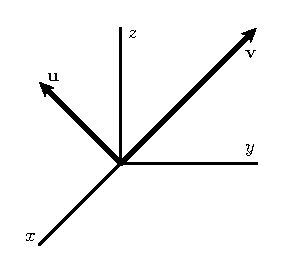
\includegraphics{figures/fig_9_4_activity_2}
        \caption{Vectors $\vu$ and $\vv$}
        \label{F:9.4.activity.2}
      \end{center}
    \end{figure}

  \item Do the vectors $\va = \langle 1,3,-2\rangle$,
    $\vb=\langle2,1,-4\rangle$, and $\vc=\langle 0, 1, 0\rangle$ lie
    in the same plane?  Use the concepts from this section to explain.
    
    \ea
\end{activity}

\begin{activitySolution}
\ba
\item The vector $\vu \times \vv$ is orthogonal to $\vu$ and $\vv$. Now
\[\vu \times \vv = \langle 3, 5, -1\rangle \times \langle 2, -2, 1\rangle = \langle 3, -5, -16 \rangle,\]
so one unit vector orthogonal to $\vu$ and $\vv$ is 
\[\vz=\frac{1}{|\vu \times \vv|} \vu \times \vv = \frac{1}{\sqrt{290}} \langle 3, -5, -16 \rangle.\]
Another unit vector orthogonal to $\vu$ and $\vv$ is $-\vz$. 

\item The volume of the parallelepiped formed by the $\vu$, $\vv$, and $\vw$ is
\[|(\vu \times \vv)\cdot \vw| = |\langle 3, -5, -16 \rangle \cdot \langle 3,3,1\rangle| = 22.\]

\item Let $P=(0,1,2)$, $Q=(4,1,0)$, and $R=(-2,2,2)$. Two vectors in the plane are $\overrightarrow{PQ} = \langle 4,0,-2 \rangle$ and $\overrightarrow{PR} = \langle -2,1,0 \rangle$. So the vector $\overrightarrow{PQ} \times \overrightarrow{PR} = \langle 2, 0, 4\rangle$ is a vector orthogonal to the plane containing the points.

\item Recall that $\vu \times \vv$ is orthogonal to $\vu$ and $\vv$ and that $\vu$, $\vv$ and $\vu \times \vv$ in that order form a right hand system. 

\item Note that $\vu \times \vv = \langle -10, 0, -5 \rangle$, and that $\vu \times \vv$ is orthogonal to every vector in the plane determined by $\vu$ and $\vv$. Now $(\vu \times \vv) \cdot \vw = 0$, so $\vw$ is in the plane determined by $\vu$ and $\vv$.  

\ea
\end{activitySolution}
\aftera
